\documentclass[9pt]{beamer}
% package list
\usepackage{./Amsterdam}
\usepackage{graphicx}
\usepackage[framemethod=TikZ]{mdframed}
\usepackage{wrapfig}
% setting 
\definecolor{MidnightBlue}{RGB}{0,103,149}

\setbeamertemplate{frametitle}{\vspace{0.2cm}\hspace{-0.5cm}\bf\insertframetitle}
\setbeamertemplate{blocks}[rounded][shadow=true]
\setbeamercolor*{title}{use=structure,fg=white,bg=structure.fg,}
\setbeamertemplate{title page}[default][colsep=-4bp,rounded=true,shadow=true]
% prensentation info
\title[Conditional Random Field: Pixel-Level Saliency Detection]
{ {Application of Conditional Random Fields in \\Pixel-Level Salient Object Detection within an Image\\using Local, Regional, and Global Features}}
\author[Jimmy Lin and Chris Claoue Long]{\bf Jimmy Lin \\Chris Claoue Long}
\institute{\bf Dr. Stephen Gould\\[0.3cm] College of Engineering and Computer Science \\Australian National University}
\date{\bf \today}
% new command definition
\DeclareMathOperator*{\argmin}{arg\,min}
\DeclareMathOperator*{\argmax}{arg\,max}
\newcommand{\SUM}{\sum\limits}
%%% beginning of document
\begin{document}
\begin{large}
\frame{\maketitle}%\titlepage}
\end{large}

%{{{ Introduction
\section{Introduction}
\frame{
    \frametitle{Introduction and Motivation}
    \begin{center}
    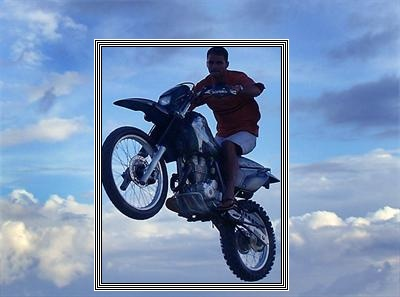
\includegraphics[width=1.6in,height=1.15in]{./intro_image/motor_label.jpg} \hspace{0.1cm}
    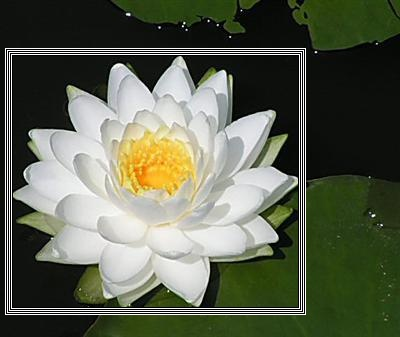
\includegraphics[width=1.6in,height=1.15in]{./intro_image/flower_label.jpg} \hspace{0.1cm} \\
    {\footnotesize Fig.1 Images from MSRA dataset B}
    \end{center}
    Saliency is the prominence of an object in an image.\\[10pt]
    Salient object detection is useful in numerous areas, for instance, in siimulating human vision by robots, augmented Reality, 3D surface reconstruction and more. \\[10pt]
    Often detected by its \textbf{high contrast boundary} to its near neighbours, \textbf{distinction from its surrounds}, \textbf{intensive colour distribution} compared to all other color component in candidate image and \textbf{space continuity of saliency}.\\[10pt]
}
%}}}

%{{{ Related Works
\section{Related Works}
\frame{
    \frametitle{Related Works}
    \begin{itemize}
        \item Salient-based Model (SM,1998) \\
        \begin{thebibliography}{9}
        \footnotesize
        \bibitem{ConcreteMath} Itti, Laurent, Christof Koch, and Ernst Niebur. "A model of saliency-based visual attention for rapid scene analysis."\textit{ Pattern Analysis and Machine Intelligence, IEEE Transactions on 20.11 (1998): 1254-1259.}
    \end{thebibliography}

    \item Fuzzy Growing Method (FG,2003) \\
        \begin{thebibliography}{9}
            \footnotesize
            \bibitem{ConcreteMath} Ma, Yu-Fei, and Hong-Jiang Zhang. "Contrast-based image attention analysis by using fuzzy growing."\textit{ Proceedings of the eleventh ACM international conference on Multimedia. ACM, 2003.} 
            \end{thebibliography}
    \item CRF-based Model (CRFM,2007)
        \begin{thebibliography}{9}
            \footnotesize 
            \bibitem{ConcreteMath} Liu, Tie, et al. "Learning to detect a salient object."\textit{ Computer Vision and Pattern Recognition, 2007. CVPR'07. IEEE Conference on. IEEE, 2007. }
            \bibitem Liu, Tie, et al. "Learning to detect a salient object."\textit{ Pattern Analysis and Machine Intelligence, IEEE Transactions on 33.2 (2011): 353-367.}
        \end{thebibliography}
    \end{itemize}
}


\frame{
    \frametitle{Evaluation Criteria}
    \begin{itemize}
        \item Region-based measurement \\
            \begin{center}
            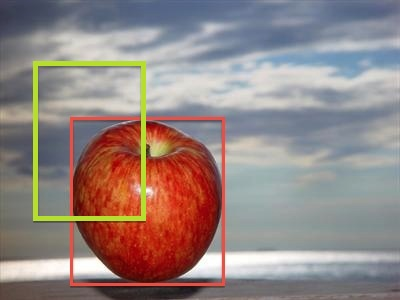
\includegraphics[width=1.0in,height=0.8in]{Picture/Creteria/A.jpg} \hspace{0.1cm}
            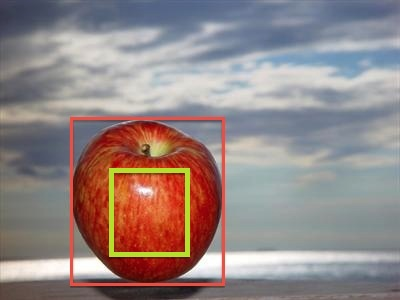
\includegraphics[width=1.0in,height=0.8in]{Picture/Creteria/B.jpg} \hspace{0.1cm}
            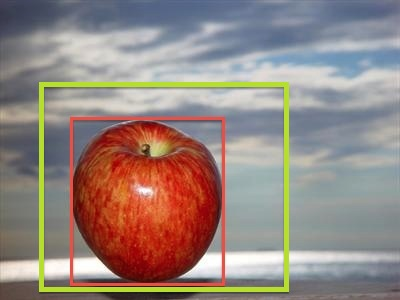
\includegraphics[width=1.0in,height=0.8in]{Picture/Creteria/C.jpg} \hspace{0.1cm} \\
            {\footnotesize (a) arbitrary labelling (b) large prec but low recall (c) large recall but low prec}
            \end{center}
            \begin{itemize}
                \item Ratio of Precision to Recall \\
                    Precision: \% of pixels that are correctly detected in ground truth\\ 
                    Recall: \% of pixels that are correctly detected in resulted detection\\
                \item F-Measure
    $$ F_{\alpha} = \frac{(1+\alpha) \times{Precision}\times{Recall}} {\alpha \times Precision + Recall} $$
            \end{itemize}
        \item Boundary-based measurement
            \begin{itemize}
                \item Boundary Displacement Error (BDE) \\
                    Measures the average of positional difference of ground truth and resulted detection.

            \end{itemize}
    \end{itemize}

            \hrule
    \begin{thebibliography}{9}
        \tiny
        \bibitem{ConcreteMath} Liu, Tie, et al. "Learning to detect a salient object."\textit{ Computer Vision and Pattern Recognition, 2007. CVPR'07. IEEE Conference on. IEEE, 2007. }
    \end{thebibliography}
}
\frame{
    \frametitle{Comparisons between Existing Approaches}
    \begin{center}
    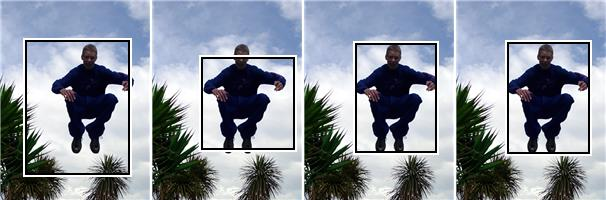
\includegraphics[width=2in,height=0.8in]{./related_work/perfectComparison/0_imCanvs_Compare.jpg} 
    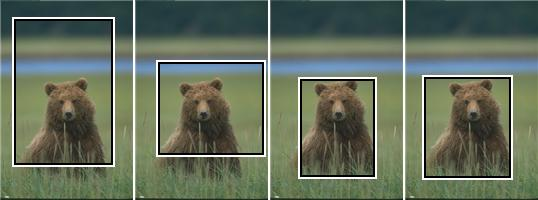
\includegraphics[width=2in,height=0.8in]{./related_work/perfectComparison/3_imCanvs_Compare.jpg} \\
    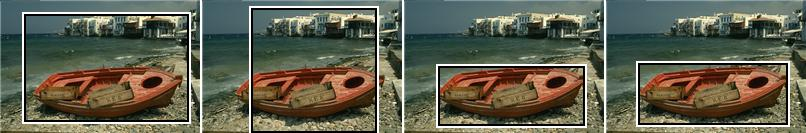
\includegraphics[width=2in,height=0.8in]{./related_work/perfectComparison/18_imCanvs_Compare.jpg} 
    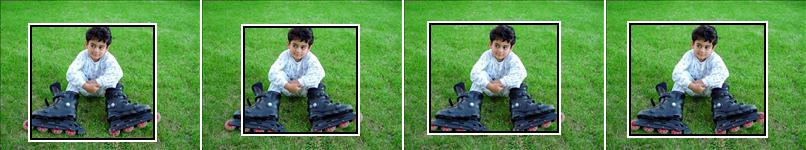
\includegraphics[width=2in,height=0.8in]{./related_work/perfectComparison/153_imCanvs_Compare.jpg} \\
    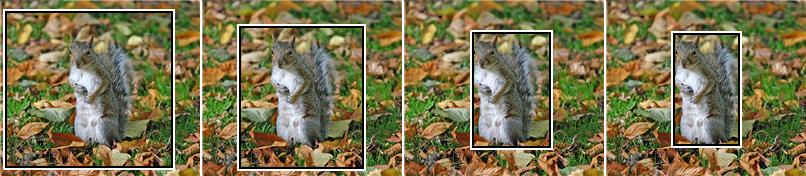
\includegraphics[width=2in,height=0.8in]{./related_work/sosoComparison/13_imCanvs_Compare.jpg} 
    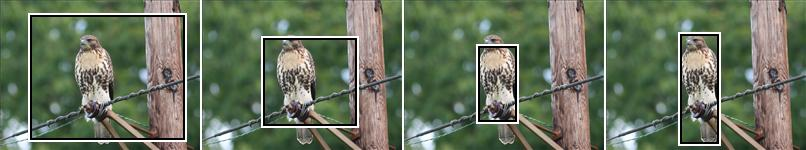
\includegraphics[width=2in,height=0.8in]{./related_work/sosoComparison/159_imCanvs_Compare.jpg} \\ 
    {\footnotesize (a) FG(Ma,2003) (b) SM(Itti,1998) (c) CRFM(Liu,2007) (d) Ground truth\vspace{0.3cm}  \\}
    \end{center}
}
%}}}

%{{{ Problem Formulation
\section{Problem Formulation}
\frame{
    \frametitle{Formulation}
    Given an image $I$, we want to compute the location of a salient object.\\[10pt]
    Binary labelling task -- for each pixel $x$, indicate whether it belongs to the salient object (1) or not (0). 
    Thus, our objective is to have corresponding map $A$, indicating binary saliency of one pixel. \\[10pt]
    \begin{center}
        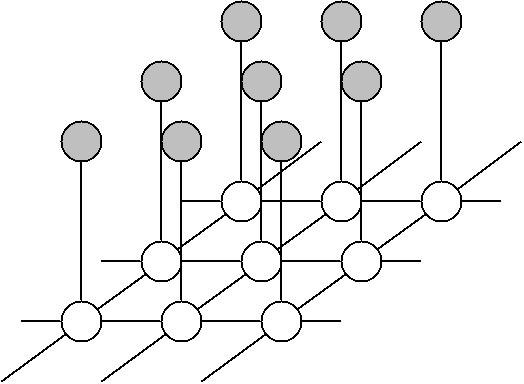
\includegraphics[width=1.8in,height=1in]{./intro_image/mrf.jpg} \\
        \footnotesize Fig.2 graph for Conditional Random Field
        \end{center}
    Build up a probabilistic model $P(A|I)=\frac{1}{Z}e^{-E(A|I)}$, where $\frac{1}{Z}$ is the normalising factor, and $E(A|I)$ is the energy function incorporating both unary and pairwise potentials between pixels.
}
    
    
%    calculate the local, regional and global features.\\
%    In our program, we used contrast (local), centre-surround histogram comparisons around potentially salient areas (regional) and the colour spatial distribution of the image (global).\\[10pt] 
%    We then run CRF inference over the outcome of these calculations, and select the region that seems most probable to be salient, effectively a winner-takes-all approach. Finally, we output a bounding box rectangle that encompasses this region.
\frame{
    \frametitle{Pairwise Feature}
    Formally, the energy function can be represented as
    $$
    E(A|I) = \SUM_x S_{unary}(a_x,I) + \lambda_0 \SUM_{x,x'}S_{pair}(a_x,a_{x'},I)
    $$
    where $\lambda$ is the relative weight between the summary of multiple unary features and pairwise features. \\[10pt]
    The pairwise feature $S(a_x,a_{x'},I)$ exploits the spatial relationship between two adjacent pixels.  It can be viewed as a ``penalty'' for labelling adjacent pixels the same or differently.
    $$
    S(a_x,a_{x'},I) = |a_x-a_{x'}| \cdot e^{-\beta d_{x,x'}}
    $$
    where $x,x'$ represent two adjacent pixels, $d_{x,x'}$ is the L2-norm (standard norm) representing the colour difference between the two pixels, and $\beta=(2\langle||I_x-I_{x'}||^2\rangle)^{-1}$ is a robust parameter to weight the colour contrast.
}
\frame{
    \frametitle{Unary Features Combination}
    The unary potential for combination of three features is specified as 
    $$
    S_{unary}(a_x,I) = \SUM_{k=1}^K \lambda_k \cdot F_k(a_x,I)
    $$
    where $\lambda_k$ is the weight of the $k^{th}$ feature conforming to $\sum_{k=1}^{K} \lambda_k = 1$.
    \begin{center}
    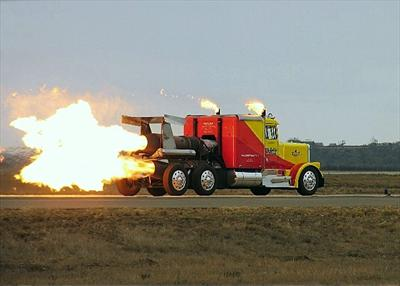
\includegraphics[width=0.72in,height=0.52in]{./MC_image/8.jpg}
    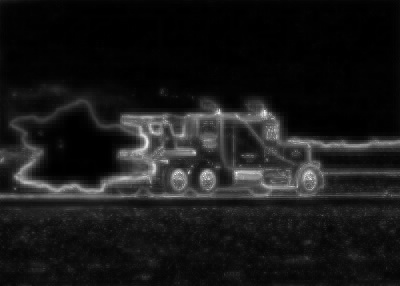
\includegraphics[width=0.72in,height=0.52in]{./MC_image/8_MC.jpg}
    %\includegraphics[width=0.72in,height=0.52in]{./MC_image/8_CSH.jpg} 
    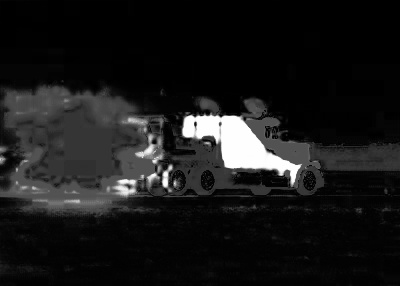
\includegraphics[width=0.72in,height=0.52in]{./MC_image/8_CSD.jpg} \\
    {\footnotesize Fig.3 Preview of feature maps}
    \end{center}
    The value of each feature $F_k(a_x,I)$ comes from a normalised feature map $f_k(x,I)\in[0,1]$, and for each pixel:
    $$
    F_k(a_x,I) = \left\{\begin{matrix}f_k(x,I), & a_x=0\\1-f_k(x,I), & a_x=1\end{matrix}\right. 
    $$
    }
%}}}

%{{{ CRF content
\section{Conditional Random Field}
\frame{
    \frametitle{Learning}
    It is technically difficult to directly compute the optimisation of the following,
    $$
    E(A|I) = \SUM_x \SUM_{k=1}^K \lambda_k \cdot F_k(a_x,I) + \lambda_0 \SUM_{x,x'}S_{pair}(a_x,a_{x'},I)
    $$
    Thus, we separate the different types of potentials to derive an approximate solution
    $$
    S_{unary}(a_x,I) = \SUM_{k=1}^K \lambda_k \cdot F_k(a_x,I)
    $$
    This can be achieved by the logistic regression. \\[10pt]
    Then we optimise $\lambda_0$ as an ordinary CRF learning task.
    $$
    E(A|I) = \SUM_x S_{unary}(a_x,I) + \lambda_0 \SUM_{x,x'}S_{pair}(a_x,a_{x'},I)
    $$
    It is somewhat similar to the Coordinate Descent Method with one iteration.
}
\frame{
    \frametitle{Inference}
    After the linear coefficient $\lambda$ is determined, we can infer the binary saliency mask of the image. \\[10pt]
    CRF inference is used to determine the assignment of binary saliency of each pixel $a_x$, which minimises the energy function
    $$
    E(A|I) = \SUM_x \SUM_{k=1}^K \lambda_k \cdot F_k(a_x,I) + \lambda_0 \SUM_{x,x'}S_{pair}(a_x,a_{x'},I)
    $$
}
%}}}

%{{{ Feature Extraction
\section{Feature Extraction}
\frame{
    \newcommand{\imageVSpacing}{\vspace*{0.5cm}}
    \frametitle{Feature Extraction}
    \begin{center}
    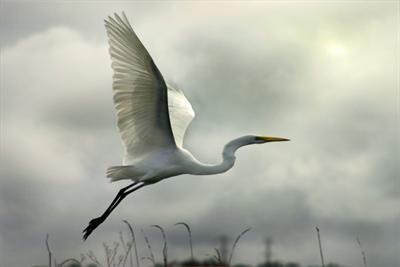
\includegraphics[width=0.72in,height=0.52in]{./MC_image/1.jpg}
    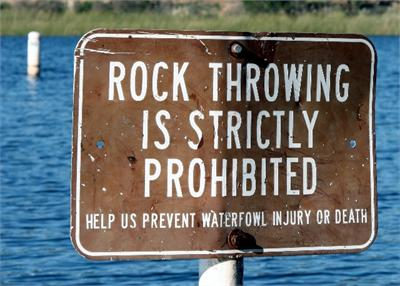
\includegraphics[width=0.72in,height=0.52in]{./MC_image/2.jpg}
    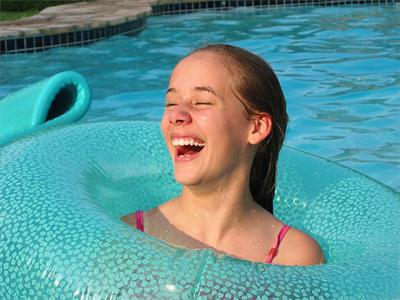
\includegraphics[width=0.72in,height=0.52in]{./MC_image/3.jpg} 
    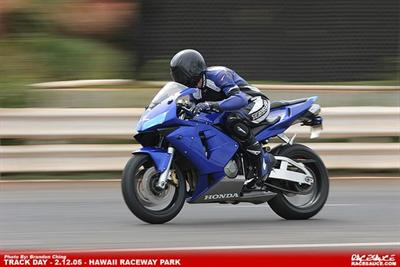
\includegraphics[width=0.72in,height=0.52in]{./MC_image/4.jpg} 
    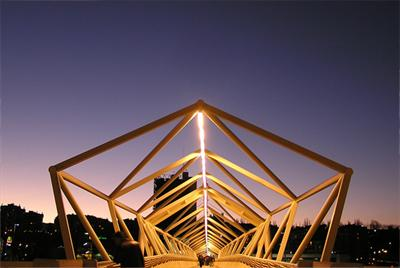
\includegraphics[width=0.72in,height=0.52in]{./MC_image/5.jpg} 
    \\
    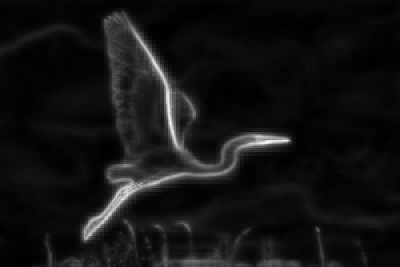
\includegraphics[width=0.72in,height=0.52in]{./MC_image/1_MC.jpg}
    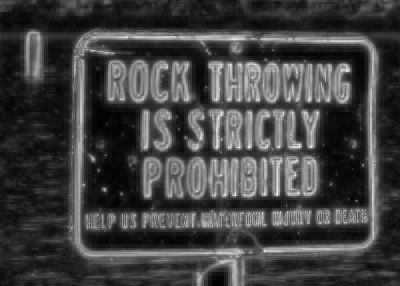
\includegraphics[width=0.72in,height=0.52in]{./MC_image/2_MC.jpg}
    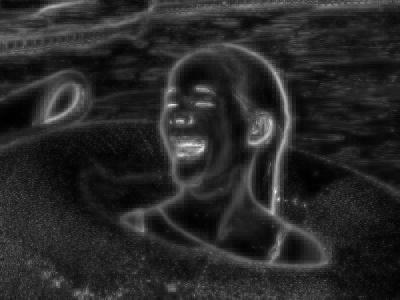
\includegraphics[width=0.72in,height=0.52in]{./MC_image/3_MC.jpg}
    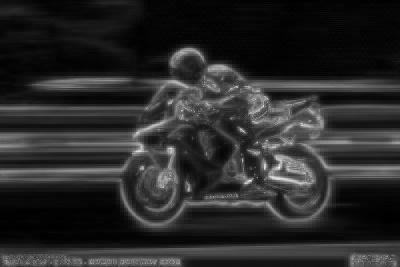
\includegraphics[width=0.72in,height=0.52in]{./MC_image/4_MC.jpg}
    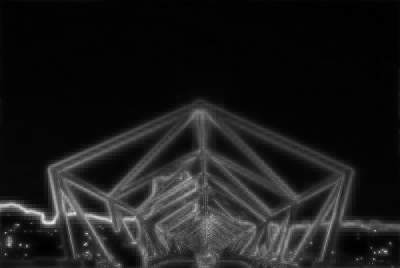
\includegraphics[width=0.72in,height=0.52in]{./MC_image/5_MC.jpg}
    \\
    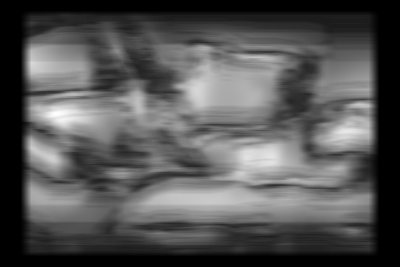
\includegraphics[width=0.72in,height=0.52in]{./MC_image/1_CSH.jpg}
    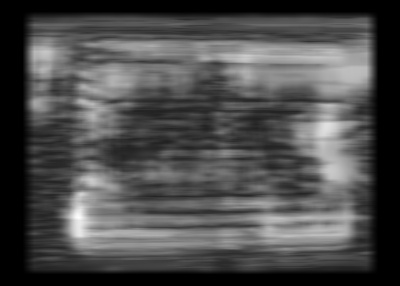
\includegraphics[width=0.72in,height=0.52in]{./MC_image/2_CSH.jpg}
    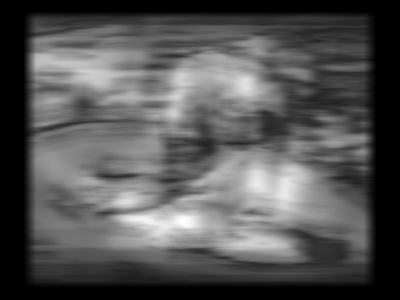
\includegraphics[width=0.72in,height=0.52in]{./MC_image/3_CSH.jpg}
    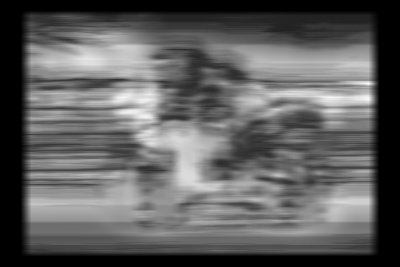
\includegraphics[width=0.72in,height=0.52in]{./MC_image/4_CSH.jpg}
    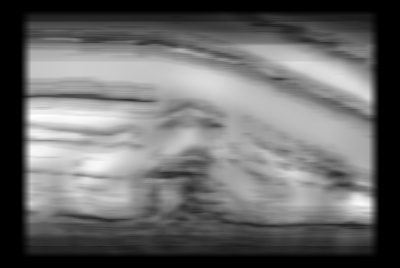
\includegraphics[width=0.72in,height=0.52in]{./MC_image/5_CSH.jpg}
    \\
    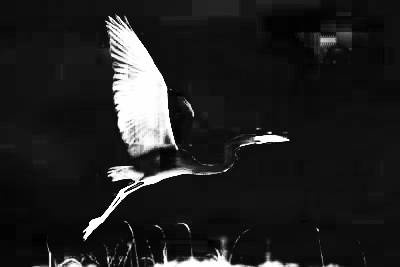
\includegraphics[width=0.72in,height=0.52in]{./MC_image/1_CSD.jpg}
    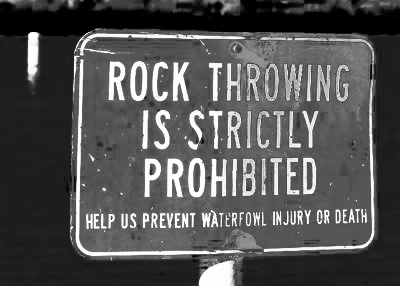
\includegraphics[width=0.72in,height=0.52in]{./MC_image/2_CSD.jpg}
    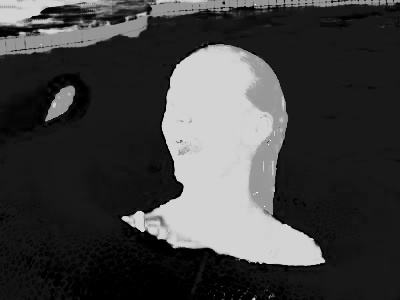
\includegraphics[width=0.72in,height=0.52in]{./MC_image/3_CSD.jpg}
    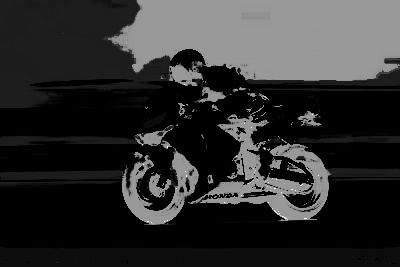
\includegraphics[width=0.72in,height=0.52in]{./MC_image/4_CSD.jpg}
    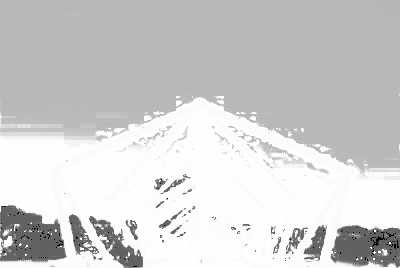
\includegraphics[width=0.72in,height=0.52in]{./MC_image/5_CSD.jpg} \\
    {\footnotesize From Top to Bottom Row: (1) Original Image (2) Local: MultiScale Contrast \\
    (3) Regional: Center-Surround Histogram (4) Global: Color Spatial Distribution}
\end{center}
}
\frame{
    \frametitle{Local: Multiscale Contrast}
    Create a contrast map from the linear combination of image contrast at all levels of an N-level gaussian image pyramid, using the pixels $x$ in the image $I$:
    $$
    f_c(x,I) = \SUM_{n = 1}^{N}\SUM_{x'\in W(x)}||I^n(x)-I^n(x')||^2
    $$
    where W(x) is a window that delineates which area to consider for neighbouring pixels to compare contrast values.\\[10pt]
    \begin{center}
    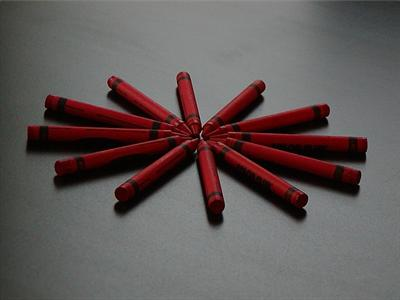
\includegraphics[width=0.8in,height=0.72in]{contrast/1orig.jpg}
    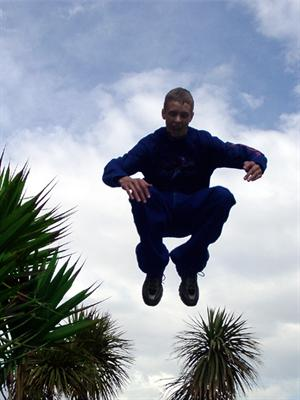
\includegraphics[width=0.8in,height=0.72in]{contrast/2orig.jpg}
    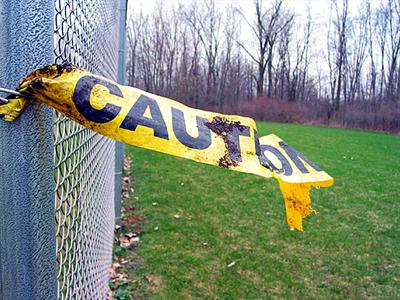
\includegraphics[width=0.8in,height=0.72in]{contrast/3orig.jpg}\\
    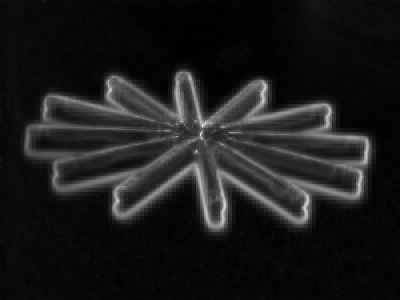
\includegraphics[width=0.8in,height=0.72in]{contrast/1cont.jpg}
    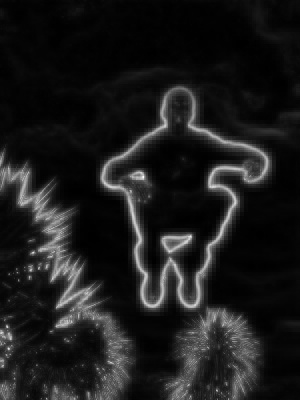
\includegraphics[width=0.8in,height=0.72in]{contrast/2cont.jpg}
    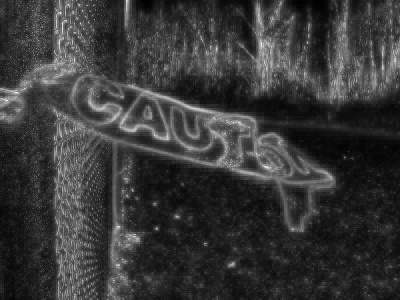
\includegraphics[width=0.8in,height=0.72in]{contrast/3cont.jpg}
    \end{center}
}
\frame{
    \frametitle{Regional: Center-Surround Histogram}
    Given a rectangle $R_s(x)$around a salient region, create a frame $R(x)$ around it so that the area of the frame is equal to that of the rectangle (this is displaced as needed to fit into the image dimensions), at a suitable aspect ratio.\\[10pt]
 \begin{center}
     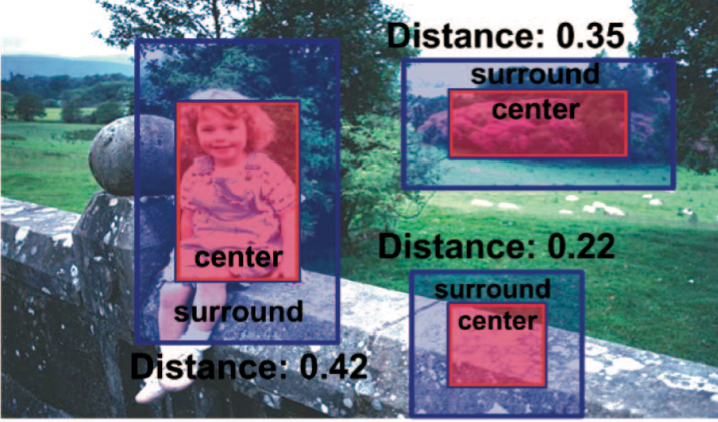
\includegraphics[width=2in,height=1in]{./hist_feature/Histogram.png} \hspace{0.1cm}
    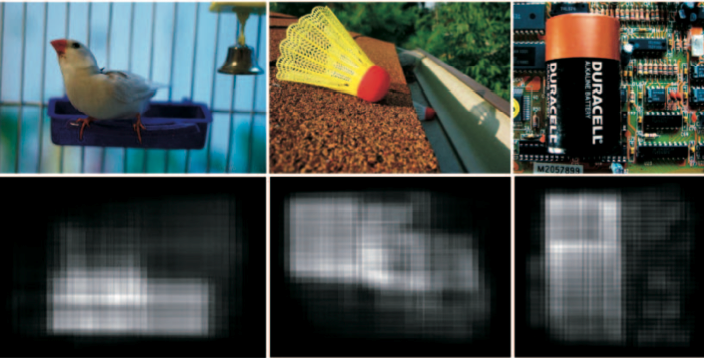
\includegraphics[width=2in,height=1in]{./hist_feature/Histogram_featuremaps.png}
    \end{center}
    \vspace{0.05cm}
    \hrule 
    \begin{thebibliography}{9}
            \tiny 
        \bibitem{ConcreteMath} Liu, Tie, et al. "Learning to detect a salient object."\textit{ Computer Vision and Pattern Recognition, 2007. CVPR'07. IEEE Conference on. IEEE, 2007. }
    \end{thebibliography}
}
\frame{
    \frametitle{Regional: Center-Surround Histogram}
    Create a colour RGB histogram for both the rectangle and the surrounding frame with a certain resolution (number of ``bins'' for each colour)\\[10pt]
%, and calculate how many pixels fall into each colour's bins in the frame and the rectangle.\\[10pt]
%    Finally, c
    Calculate the $\chi^2$ value between the two histograms to obtain the differences between the rectangle and the surrounding frame.  Do this for multiple aspect ratios, and keep the largest $\chi^2$ value: %and the frame that formed it:
    $$
    R(x) = \argmax\limits_{R(x)}\chi^2(R(x), R_s(x)) =\argmax\limits_{R(x)}\frac{1}{2}\cdot\SUM_{i\in bins}\frac{(hist_{R(x)_i}-hist_{R_s(x)_i})^2}{hist_{R(x)_i}+hist_{R_s(x)_i}}
    $$
    The center-surround histogram feature is finally calculated as:
    $$
    f_h(x,I)\propto\SUM_{x'|x\in R(x')}w_{xx'}\chi^2(R(x'),R_s(x'))
    $$
}

\frame{
    \frametitle{Global: Colour Spatial Distribution}
    Create a Gaussian Mixture Model to compute the spatial variance and continuity of colour in an image.\\[10pt]
    The component model is created from only a subset of the pixels in the image, and the maximum number of iterations is limited in order to reduce the time taken to compute this feature without sacrificing too much accuracy.\\[10pt]
    \begin{center}
    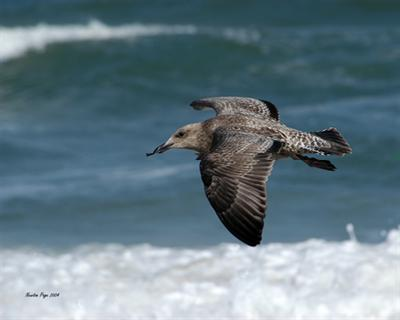
\includegraphics[width=0.72in,height=0.52in]{./CSD_image/1.jpg}
    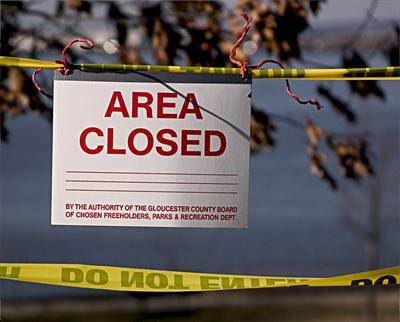
\includegraphics[width=0.72in,height=0.52in]{./CSD_image/2.jpg}
    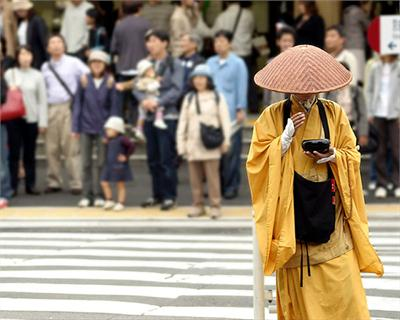
\includegraphics[width=0.72in,height=0.52in]{./CSD_image/3.jpg}\\
    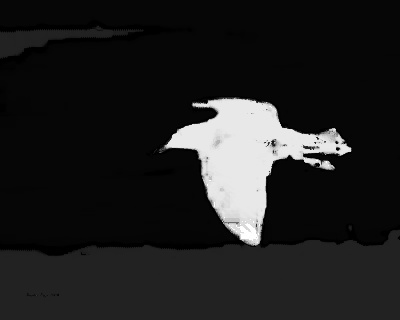
\includegraphics[width=0.72in,height=0.52in]{./CSD_image/1_CSD.jpg}
    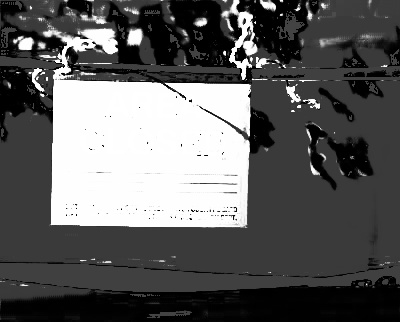
\includegraphics[width=0.72in,height=0.52in]{./CSD_image/2_CSD.jpg}
    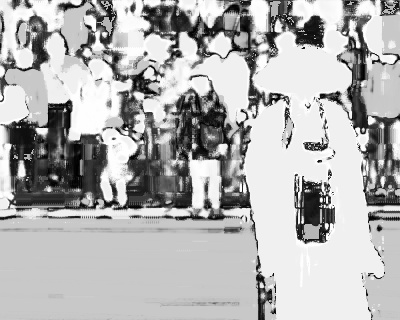
\includegraphics[width=0.72in,height=0.52in]{./CSD_image/3_CSD.jpg}
    \end{center}
}
\frame{
    \frametitle{Global: Colour Spatial Distribution}
    Each pixel is associated to a colour component with the probability
    $$
    P(c|I_x) = \frac{\omega_c\mathcal{N}(I_x|\mu_c,\sigma_c)}{\SUM_c \omega_c \mathcal{N}(I_x|\mu_c,\Sigma_c)}
    $$
    where $\omega_c$ is the weight, $\mu_c$ is the mean colour, $\sigma_c$ is the covariance, and $\mathcal N(I_x|\mu_c,\sigma_c)$ is the multivariate normal distribution of the $c^{th} component$\\[10pt]
    The final colour spatial distribution feature is defined as a weighted sum:
    $$
    f_s(x,I)\propto\SUM_c p(c|I_x)\cdot(1-V(c))
    $$
    where $V(c)$ is the normalised covariance (horizontal and vertical variances) of the $c^{th}$ component, contained between 0 and 1.
}


%}}}

%{{{ Epilogue
\frame{
    \frametitle{Our variations to previous works}
    Separate learning of parameters in the CRF model\\[10pt]
    Improved speed and performance of the given feature extraction processes
    \begin{itemize} 
    \item Reducing the resolution of the image before calculating its colour spatial distribution, and limiting the complexity of the gaussian model fitting without reducing overall quality of the feature map:
    \item Accounting for center-surround histograms that would otherwise exceed the boundary of the image, especially in corners
    \item Improved calculation of the aspect ratio to use when calculating the center-surround histogram frame
    \end{itemize}
}
\section{Epilogue}
\frame{
    \frametitle{Our Project Progress}
    \begin{center}
        \includegraphics[width=0.72in,height=0.52in]{./aknowledgement/5_157_157174Origin.jpg}
        \includegraphics[width=0.72in,height=0.52in]{./aknowledgement/5_157_157174MC.jpg}
        \includegraphics[width=0.72in,height=0.52in]{./aknowledgement/question.jpg}
        \includegraphics[width=0.72in,height=0.52in]{./aknowledgement/5_157_157174CSD.jpg}
        \includegraphics[width=0.72in,height=0.52in]{./aknowledgement/question.jpg}
        \includegraphics[width=0.72in,height=0.52in]{./aknowledgement/5_157_157174Label.jpg} \\
        \includegraphics[width=0.72in,height=0.52in]{./aknowledgement/5_161_161904Origin.jpg}
        \includegraphics[width=0.72in,height=0.52in]{./aknowledgement/5_161_161904MC.jpg}
        \includegraphics[width=0.72in,height=0.52in]{./aknowledgement/question.jpg}
        \includegraphics[width=0.72in,height=0.52in]{./aknowledgement/5_161_161904CSD.jpg}
        \includegraphics[width=0.72in,height=0.52in]{./aknowledgement/question.jpg}
        \includegraphics[width=0.72in,height=0.52in]{./aknowledgement/5_161_161904Label.jpg} \\
        \includegraphics[width=0.72in,height=0.52in]{./aknowledgement/5_162_162166Origin.jpg}
        \includegraphics[width=0.72in,height=0.52in]{./aknowledgement/5_162_162166MC.jpg}
        \includegraphics[width=0.72in,height=0.52in]{./aknowledgement/question.jpg}
        \includegraphics[width=0.72in,height=0.52in]{./aknowledgement/5_162_162166CSD.jpg}
        \includegraphics[width=0.72in,height=0.52in]{./aknowledgement/question.jpg}
        \includegraphics[width=0.72in,height=0.52in]{./aknowledgement/5_162_162166Label.jpg} \\
        {\footnotesize Fig.5 Our implementation}
    \end{center}
}
\frame{
    \frametitle{Thank you! Questions?}
    \begin{center}
        \includegraphics[width=0.72in,height=0.52in]{./aknowledgement/5_157_157174Origin.jpg}
        \includegraphics[width=0.72in,height=0.52in]{./aknowledgement/5_157_157174MC.jpg}
        \includegraphics[width=0.72in,height=0.52in]{./aknowledgement/question.jpg}
        \includegraphics[width=0.72in,height=0.52in]{./aknowledgement/5_157_157174CSD.jpg}
        \includegraphics[width=0.72in,height=0.52in]{./aknowledgement/question.jpg}
        \includegraphics[width=0.72in,height=0.52in]{./aknowledgement/5_157_157174Label.jpg} \\
        \includegraphics[width=0.72in,height=0.52in]{./aknowledgement/5_161_161904Origin.jpg}
        \includegraphics[width=0.72in,height=0.52in]{./aknowledgement/5_161_161904MC.jpg}
        \includegraphics[width=0.72in,height=0.52in]{./aknowledgement/question.jpg}
        \includegraphics[width=0.72in,height=0.52in]{./aknowledgement/5_161_161904CSD.jpg}
        \includegraphics[width=0.72in,height=0.52in]{./aknowledgement/question.jpg}
        \includegraphics[width=0.72in,height=0.52in]{./aknowledgement/5_161_161904Label.jpg} \\
        \includegraphics[width=0.72in,height=0.52in]{./aknowledgement/5_162_162166Origin.jpg}
        \includegraphics[width=0.72in,height=0.52in]{./aknowledgement/5_162_162166MC.jpg}
        \includegraphics[width=0.72in,height=0.52in]{./aknowledgement/question.jpg}
        \includegraphics[width=0.72in,height=0.52in]{./aknowledgement/5_162_162166CSD.jpg}
        \includegraphics[width=0.72in,height=0.52in]{./aknowledgement/question.jpg}
        \includegraphics[width=0.72in,height=0.52in]{./aknowledgement/5_162_162166Label.jpg} \\
        {\footnotesize Fig.5 Our implementation}
    \end{center}
}
%}}}

%{{{ Reference
\section{References}
\frame{
    \frametitle{References}
    \begin{thebibliography}{9}
        \bibitem{ConcreteMath} Liu, Tie, et al. "Learning to detect a salient object."\textit{ Computer Vision and Pattern Recognition, 2007. CVPR'07. IEEE Conference on. IEEE, 2007. }
        \bibitem{ConcreteMath} Liu, Tie, et al. "Learning to detect a salient object."\textit{ Pattern Analysis and Machine Intelligence, IEEE Transactions on 33.2 (2011): 353-367.}
        \bibitem{ConcreteMath} Itti, Laurent, Christof Koch, and Ernst Niebur. "A model of saliency-based visual attention for rapid scene analysis."\textit{ Pattern Analysis and Machine Intelligence, IEEE Transactions on 20.11 (1998): 1254-1259.}
        \bibitem{ConcreteMath} Ma, Yu-Fei, and Hong-Jiang Zhang. "Contrast-based image attention analysis by using fuzzy growing."\textit{ Proceedings of the eleventh ACM international conference on Multimedia. ACM, 2003.} 
        \bibitem{ConcreteMath} Stephen Gould, "DARWIN: A Framework for Machine Learning and Computer Vision Research and Development", \textit{Journal of Machine Learning Research (JMLR), 13(Dec):3533−3537, 2012}.
    \end{thebibliography}
}
%}}}

\end{document}
